\documentclass[12pt]{article}

\usepackage[utf8]{inputenc}
\usepackage[brazil]{babel}
\usepackage[a4paper, left=3cm, right=2cm, top=3cm, bottom=2cm]{geometry}
\usepackage[backend=biber, style=alphabetic, sorting=ynt]{biblatex}
\usepackage{setspace}
\usepackage{graphicx}
\usepackage{csquotes}
\usepackage{helvet}

\renewcommand{\familydefault}{\sfdefault}

\graphicspath{{./src/img/}}
\addbibresource{references.bib}

\title{Uma abordagem moderna de Monorepos}
\author{Gabriel Saito \and Matheus Moreira}
\date{Novembro 2022}

\begin{document}
  \maketitle

  \newpage
  \tableofcontents
  \onehalfspacing

  \nocite{*}

  \section{Introdução}

Quando falamos de desenvolvimento, parte importante da construção de um bom software é o armazenamento e versionamento do código, então visando suprir essa necessidade surgem os repositórios, que atendem essa necessidade do projeto ao longo de sua fase de desenvolvimento. Se tratando de repositórios temos três abordagens principais, a abordagem de Monorepo, Multirepo e Monolítica. A abordagem de Multirepo utiliza vários repositórios onde são hospedadas as diversas partes que compõem uma ou mais aplicações. O Monorepo, que surge com uma abordagem oposta, onde todas as partes que compões uma ou mais aplicações, ao invés de ficarem separadas em diferentes repositórios, ficam sob um único repositório, trazendo assim uma série de vantagens, como a possibilidade de reutilização de código, fácil padronização de projetos, e a facilidade de executar todas as partes separadas da aplicação de uma forma única e concisa. 

  \section{O que é um Monorepo}

Um Monorepo é uma arquitetura para repositórios de código versionado de projetos, que tem como objetivo centralizar as diversas aplicações e pacotes de uma empresa em um único repositório, podendo elas serem relacionadas ou independentes e gerenciadas por um único ou diversos times dentre desta empresa. 

Algumas empresas utilizam a arquitetura de Monorepo para manter uma única fonte de verdade entre todas as aplicações e pacotes da organização centralizadas. Os Monorepos são normalmente grandes em termos de espaço de armazenamento, alguns dos maiores Monorepos são de grandes empresas como Google, Microsoft, Facebook e Twitter, sendo o Monorepo da Google, em 2016, estimado em cerca de 80TBs (Terabytes), pois houve a decisão logo no início da companhia, que esta seria a sua cultura de desenvolvimento, além de possuírem ferramentas internas que foram desenvolvidas para gerenciar o repositório tendo a cultura da empresa em mente. Este Monorepo é considerado um caso de sucesso e continuam até hoje hospedando cerca de 95\% de suas aplicações neste repositório. 

Existem diversas vantagens em se ter projetos e bibliotecas centralizadas em um único repositório, principalmente quando falamos de compartilhamento de código. Vários projetos web tendem a ser compostos de componentes bases, como botões e campos de texto, em um Monorepo é fácil manter um único componente e disponibilizá-lo para todas as aplicações que vivem dentro do Monorepo, minimizando as chances de código redundante.


Monorepos podem também ser chamados de Repositórios Monolíticos, porém não devem ser confundidos com Arquitetura Monolítica, onde consiste em ter todas as funcionalidades e contexto da aplicação juntas e interligadas, sem uma separação clara entre os contextos.
  \section{O que são repositorios}

Um repositório de código é um histórico do código sendo trabalhado, podendo conter outros artefatos além do próprio código, como por exemplo, documentações, exemplos, referencias, entre outros. 

Um repositório de código não é obrigatório para o sucesso de um projeto, porém a utilização de um é considerada essencial entre os desenvolvedores, sendo extremamente raro projetos de larga escala que não possuem um repositório. 

O repositório além de observar as alterações realizadas no código, versiona essas alterações, sendo possível consultá-las futuramente. 

Existem várias formas de se utilizar um repositório, porém a mais comum é através de serviços de hospedagem de repositórios, como GitHub, GitLab e BitBucket, cada um possuindo suas peculiaridades, mas em essência todos tem como Base o Git, que é um sistema de controle de versões distribuído, que é o sistema usado por debaixo dos panos por estes serviços de hospedagem de repositórios.  
  \section{Monorepo Vs. Multirepo Vs. Monolito}

Cada arquitetura de repositórios possui suas vantagens e desvantagens, e não podemos considerar uma solução como sendo a melhor ou pior de todas, cada escopo de projeto ou empresa se adequa a um tipo de arquitetura, e é importante que seja analisado cuidadosamente cada uma antes de se iniciar um projeto, porém sempre é possível migrar de arquitetura caso seja necessário.  

Um Monorepo consiste em um único repositório contendo todas as aplicações de uma organização centralizada. Por ter suas aplicações centralizadas, automaticamente se torna disponível para todos os times, ou seja, qualquer funcionalidade ou componente desenvolvido em uma aplicação, pode ser usado por outro time em outra aplicação, como uma espécie de biblioteca que esta constantemente atualizada, tendo qualquer alteração refletida em todas as demais aplicações que consomem esta funcionalidade, evitando assim as famosas breaking changes, uma vez que quando as mudanças são aplicadas e conflitos são corrigidos antes de ser realizado o commit, não existirão mudanças que quebrem as aplicações. 

Um Multirepo, também conhecido como Polirepo, é uma arquitetura de para repositórios de código versionado de projetos mais comummente utilizado entre os times de desenvolvedores. Uma arquitetura de Multirepo é usada quando existem diversos projetos e diversos times, cada um com seu repositório separando as responsabilidades de cada aplicação em seu repositório. Multirepos não devem ser confundidos com Arquitetura de Micro serviços, uma vez que um projeto dentro de Multirepos podem ou não depender ou estar relacionado a outros projetos. 

O motivo de diversas empresas adotarem a arquitetura de Multirepo é para poder separar as responsabilidades entre times, onde cada produto ou aplicação fica sob responsabilidade de um time, e esse time trabalha apenas em seu repositório, dessa maneira as alterações em um repositório não afetam outro repositório. 

Imagine um cenário onde um time A desenvolve uma aplicação para um mercado, e um time B desenvolve uma aplicação para uma barbearia, ambos são produtos diferentes, porém podem possuir componentes comuns entre eles, como por exemplo, um botão, imagine que tanto o time A quanto o time B criem seus botões, e ambos os botões são idênticos, mesmo design e funcionalidade. Caso seja encontrado um bug, ou caso seja necessário realizar uma modificação nos botões, cada time será responsável por fazer as mesmas alterações em seus respectivos botões. Essa prática gera duplicação de código, fazendo com que tempo e, por consequência, dinheiro seja desperdiçado com um simples botão. Agora imagine que um terceiro time C, se propõem a desenvolver uma biblioteca de botões que serão compartilhados entre os times A e B, será necessário um novo repositório para que o time C possa trabalhar em seus botões, totalizando assim em três repositórios, um para cada time, cada um desses repositórios tem sua própria pipeline de testes, build e publicação. E conforme mais repositórios forem surgindo, mais complexo se torna o gerenciamento e a habilidade de compartilhar código entre os demais projetos. 

Ao implementar a arquitetura de Monorepo, todas as aplicações e bibliotecas ficam no mesmo repositório, fazendo com que tudo que seja desenvolvido dentro do repositório, automaticamente se torna disponível para qualquer time  implementar em seu projeto, além de, toda e qualquer alteração nas bibliotecas, serem refletidas imediatamente em todas as aplicações que as utilizam, evitando as famosas “breaking changes”, uma vez que quando as mudanças são aplicadas antes de ser realizado o commit, não existira uma mudança que quebre as aplicações. 

Já uma arquitetura Monolítica consiste em uma única aplicação que “faz tudo”, sendo mais comum em projetos legado, em uma arquitetura monolítica, conforme for necessário adicionar novas funcionalidades, é criado de forma interligada com a aplicação, dificultando a sua reutilização em outros projetos 
  \section{Monorepos em ambiente de produção}

Existem diversas estratégias para a implementação de projetos construídos em Monorepos no ambiente de produção, uma delas sendo com a implementação de containers usando Docker. 

Docker é uma ferramenta de plataforma aberta para o desenvolvimento e execução de aplicações, permitindo a separação das aplicações, de sua infraestrutura, sendo possível a entrega de software com maior agilidade. Com Docker é possível gerenciar sua infraestrutura da mesma forma que é gerenciada a aplicação, criando containers de forma efêmera para que possam ser executados sem a necessidade de provisionar uma máquina virtual. Em essência, Docker permite que você crie container encapsulando sua aplicação, de forma modular, permitindo que sejam orquestrados para se comunicarem uns com os outros ou de forma isolada. 

Ao adicionar a aplicação em um container, é comum encontrar situações em que cada container é um repositório, contendo seu Dockerfile específico. No entanto em Monorepos, ore termos todas as aplicações e suas dependências em um único repositório, pode ocasionar em dificuldades durante a orquestração destes containers. 

Um dos principais fatores que podem causar problemas, são as dependências locais do Monorepo, elas são normalmente bibliotecas desenvolvidas internamente no Monorepo para serem reutilizadas entre os demais projetos, cada aplicação quando passa por sua pipeline de build, necessita que todas as dependências sejam copiadas para dentro do container. Uma possível solução é organizar todas essas bibliotecas em uma única pasta e para cada aplicação copiar todas as bibliotecas para cada um dos containers, porém esta solução não é escalável, uma vez que a cada nova biblioteca adicionada ao Monorepo, o tempo de build para cada imagem cresce exponencialmente. 

Um cenário mais escalável é que durante o processo de build das aplicações, as dependências internas sejam tratadas como se fossem pacotes, baixados de uma CND (Content Delivery Network), e caso não sejam encontradas, então realizar o processo de build e publish deste pacote, dessa maneira garantindo que os pacotes sempre serão buildados durante a criação das imagens, porem passando por este fluxo apenas uma vez, sendo possível as demais aplicações apenas baixarem desta CDN a biblioteca recém buildada. 

É importante que as empresas que adotem o Monorepo em sua cultura de desenvolvimento, tenham um fluxo bem definido para o processo das imagens Docker, uma vez que este é um processo que demanda tempo, e se não for devidamente implementado, irá gerar custos buildando pacotes redundantes 
  \section{Monorepo da Google}

Desde o seu início, os desenvolvedores da Google decidiram trabalham centralizando todas as suas aplicações e serviços em um único repositório, e mesmo com o constante crescimento da empresa, e por consequência, o número de desenvolvedores, a arquitetura de Monorepo ainda é utilizada em grande força. Em 2016, foi estimado que o Monorepo da Google se aproximava de 86TBs de dados e cerca de 35 milhões de commits entre os 18 anos de existência do repositório. Devido ao imenso tamanho deste repositório, em 2012 foi necessário o desenvolvimento de ferramentas especializadas para poder gerenciar o repositório. 

A ferramenta desenvolvida para gerenciar o Monorepo recebeu o codinome Piper, de acordo com a Google, não existia uma ferramenta comercialmente disponível que conseguisse lidar com o seu Monorepo. Piper é responsável por hospedar um único repositório implementado sob a infraestrutura da google, e é distribuído entre 10 data centers ao redor do mundo. 
  \section{Ferramentas de Monorepo}

É necessário desenvolver uma ferramenta tão complexa quanto a da Google para poder implementar a arquitetura de Monorepos? Não, existem diversas ferramentas para construir e gerenciar Monorepos, dentro do ecossistema de Javascript/TypeScript algumas das ferramentas com maior índice de satisfação são: 

\begin{figure}[t]
  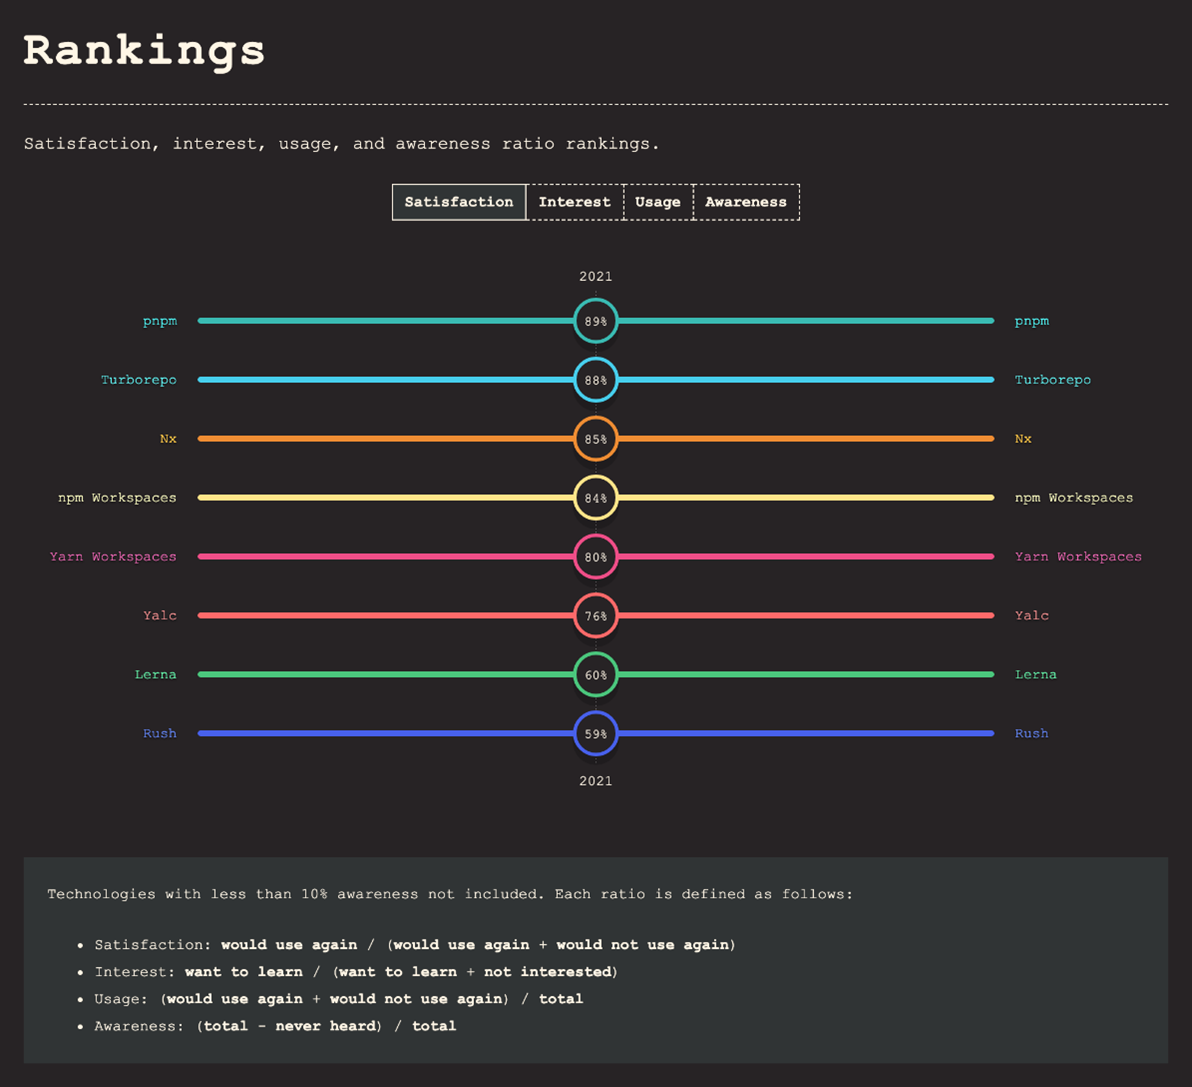
\includegraphics{monorepo-tools.png}
  \centering
  \caption{https://2021.stateofjs.com/en-US/libraries/monorepo-tools}
\end{figure}

Dentre essas ferramentas, uma que vem chamando bastante atenção recentemente é o Turborepo, uma ferramenta desenvolvida por Jared Palmer e que foi adquirida pela empresa Vercel em 2021, e possui diversas funcionalidades para facilitar o gerenciamento de Monorepos além de disponibilizar um registry para salvar o cache de builds de aplicações e pacotes, sendo o complemento ideal para o desenvolvimento de Monorepos rápidos com containers.

O Turborepo é um sistema para gerenciamento de Monorepos em ambientes Javascript e TypeScript, sendo altamente performático, possui diversas ferramentas para alavancar o desenvolvimento com a arquitetura de Monorepos, como por exemplo execuções paralelas, cache em cloud, processos de build incrementais, pipelines para execuções de tarefas, entre outras.

  \section{Cultura Monorepo}

Como tudo na área de tecnologia, Monorepo não pode ser considerado uma resposta definitiva, uma solução única para todo e qualquer problema, mas sim como uma possível solução para problemas de organização de repositórios e compartilhamento de código. Para que se obtenha sucesso na implementação de Monorepos, é importante que a organização que estiver implementando o Monorepo, esteja preparada para aderir a cultura Monorepo.

O que é a cultura Monorepo? Todos os desenvolvedores estão trabalhando em um único repositório contendo diversos projetos, é importante que haja uma comunicação clara entre os times, para evitar que uma alteração afete o trabalho dos demais. Possuir as aplicações com planos de testes consistentes, para garantir que toda e qualquer mudança não gere problemas para as aplicações. Essas são algumas das bases fundamentais para que a adoção de Monorepos se torne algo produtivo, se os times não estiverem dispostos a trabalharem de acordo com as bases, a implementação do Monorepo que inicialmente tinha o propósito de trazer benefícios para a organização, acaba por se tornar um empecilho 


  \newpage
  \printbibliography
\end{document}